% Methodology working draft: explanatory prose restored, with current notebook methods.
% To incorporate into a report, copy the body between the marked comments,
% remove the local counter setup, and use the report's own numbering.
\documentclass[11pt,a4paper]{article}
\usepackage[T1]{fontenc}
\usepackage[utf8]{inputenc}
\usepackage[margin=25mm]{geometry}
\usepackage{lmodern}
\usepackage{microtype}
\usepackage{amsmath}
\usepackage{array,booktabs,tabularx}
\usepackage{tikz}
\usetikzlibrary{arrows.meta,positioning}
\usepackage{xurl}
\usepackage[hidelinks]{hyperref}
\usepackage{caption}
\captionsetup{font=small,labelfont=bf}
\setlength{\parindent}{0pt}
\setlength{\parskip}{0.6em}
\setlength{\emergencystretch}{3em}
\renewcommand{\arraystretch}{1.2}
\newcolumntype{Y}{>{\raggedright\arraybackslash}X}
\renewcommand{\thetable}{5.\arabic{table}}
\renewcommand{\thefigure}{5.\arabic{figure}}
\hypersetup{pdftitle={Methodology working draft},pdfauthor={Yeshlen Moodley}}
\begin{document}
\setcounter{section}{4}
% BEGIN METHODOLOGY BODY

\section{Methodology}

\subsection{Research approach and design}

This study investigated whether behavioural risk scoring could identify cardless cash withdrawal transactions associated with social-engineering scams. A pragmatic epistemological stance was used because the research concerned a practical banking security problem and the development of a prototype to address it. This emphasis on useful knowledge was consistent with the principles of pragmatism described by \href{https://doi.org/10.1177/2059799120937242}{Kelly and Cordeiro (2020)}. A quantitative approach then allowed the scoring methods to be compared through their detection results and false alerts.

The research followed a design science approach, which connects the development of an artefact with an evaluation of how well it addresses the problem (\href{https://doi.org/10.1007/978-3-030-46781-4_1}{vom Brocke, Hevner and Maedche, 2020}). In this study, the artefact was a prototype that generated banking events, extracted behavioural features, calculated risk scores and presented alerts. A controlled computational experiment was used to compare rules, anomaly detection and a hybrid on the same simulated activity. The feature analysis addressed the question of relevant behavioural indicators, while the model comparison examined detection effectiveness. The dashboard demonstrated how an alert could support further review, although the effect of an intervention on customers was outside the experiment.

\subsection{Research process}

The prototype was implemented as a pipeline from customer activity to risk scores and alerts. A configuration file defined the customer population, product limits, legitimate behaviour and scam scenarios. The simulator used these settings to produce an event log, which was replayed by the feature extractor to calculate the information available for each voucher. The scoring methods then used these features to assign risk scores, and the known simulation labels allowed their decisions to be evaluated.

Figure~\ref{fig:pipeline} shows how these parts were connected. Ground truth followed a separate path because it was needed to assess the scores, but was excluded from the inputs used to fit the anomaly models. Validation labels were used to choose model settings and alert thresholds. This distinction allowed the experiment to investigate fitting without confirmed scam labels while still assessing the resulting alerts.

\begin{figure}[htbp]
\centering
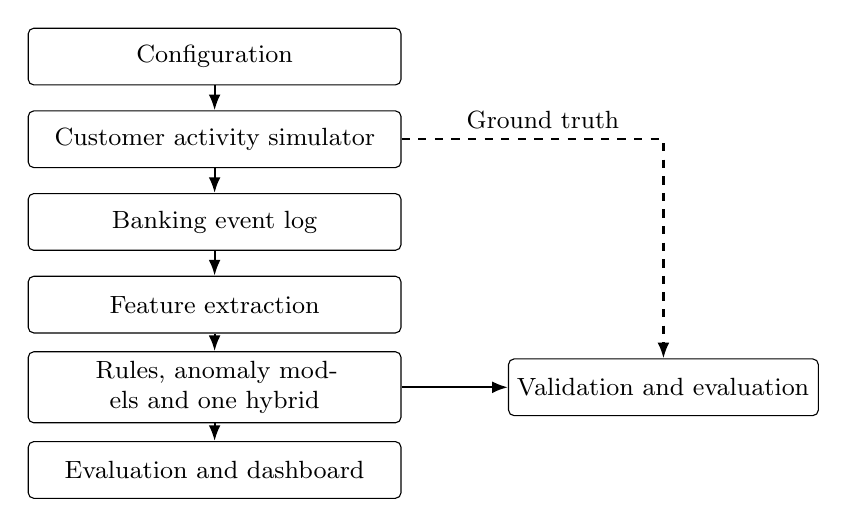
\begin{tikzpicture}[
 box/.style={draw,rounded corners=2pt,align=center,text width=4.5cm,minimum height=0.72cm,font=\small},
 arrow/.style={-{Latex[length=2mm]},thick}]
\node[box] (config) at (0,0) {Configuration};
\node[box] (sim) at (0,-1.05) {Customer activity simulator};
\node[box] (log) at (0,-2.1) {Banking event log};
\node[box] (features) at (0,-3.15) {Feature extraction};
\node[box] (scores) at (0,-4.2) {Rules, anomaly models and one hybrid};
\node[box] (dash) at (0,-5.25) {Evaluation and dashboard};
\node[box,text width=3.7cm] (validation) at (5.7,-4.2) {Validation and evaluation};
\draw[arrow] (config)--(sim);
\draw[arrow] (sim)--(log);
\draw[arrow] (log)--(features);
\draw[arrow] (features)--(scores);
\draw[arrow] (scores)--(dash);
\draw[arrow] (scores)--(validation);
\draw[arrow,dashed] (sim.east) -| node[pos=0.27,above,font=\small]{Ground truth} (validation.north);
\end{tikzpicture}
\caption{The research pipeline. Ground truth supports model selection and evaluation but is excluded from anomaly-model fitting.}
\label{fig:pipeline}
\end{figure}

Python, NumPy and pandas were used for simulation and data processing, scikit-learn for modelling, Matplotlib for the figures and Streamlit for the dashboard. Three notebooks organised the analysis: the first covered data checks and exploratory data analysis (EDA), the second fitted models and selected settings on validation data, and the third evaluated the fixed choices and prepared the dashboard results. Reusable modules supplied the simulator, feature extractor and scoring functions. The simulator seed was 42 and the model seed was 0; these were retained with the configuration and software versions to support repeatability.

\subsection{Synthetic dataset}

The study used synthetic banking activity because no real customer transaction dataset was available for this research. Rather than generating independent transaction rows, the simulator represented customers with their own habits and produced their activity over time. This was necessary because features such as a customer's usual voucher amount or whether a recipient had been used before required an actual sequence of earlier events.

A seeded, rule-based simulation was used to create this history. Each customer generated their own banking events, including app sessions, account changes, voucher creation and redemption. Voucher redemption refers to the recipient withdrawing the funds using the voucher. Customers were simulated independently, so the implementation did not represent transfers between customer agents or a network of fraudsters. The focus was the behaviour surrounding a cardless withdrawal from the sending customer's perspective.

\subsubsection*{Customer profiles and legitimate behaviour}

The simulator created 20,000 customers across four segments: students, salaried customers, customers with informal income and pensioners. Table~\ref{tab:method-1} gives the starting settings for each segment. These were simulation assumptions rather than estimates obtained from a bank. Individual activity rates and typical amounts varied around the segment values, allowing customers in the same segment to behave differently.

\begin{table}[htbp]
\centering\small
\caption{Starting customer segment settings. Monthly rate refers to voucher frequency.}
\label{tab:method-1}
\begin{tabularx}{\linewidth}{Yrrr}
\toprule
\textbf{Segment} & \textbf{Share} & \textbf{Monthly rate} & \textbf{Typical amount} \\
\midrule
Student & 20\% & 0.5 & R300 \\
Salaried & 45\% & 0.8 & R800 \\
Informal income & 20\% & 1.2 & R600 \\
Pensioner & 15\% & 0.4 & R500 \\
\bottomrule
\end{tabularx}
\end{table}

Each customer also received a home location, account opening date, preferred activity time and recurring recipients. Payday, weekend and December multipliers changed voucher frequency across the observation period, which covered 180 days from 1 July to 27 December 2025. Scam episodes were introduced only from day 30, allowing an initial period for customer history to develop.

Legitimate activity included ordinary voucher use and three unusual episodes: an emergency payment, use after a new phone was registered, and a payment redeemed while travelling. Ordinary activity could also involve new recipients, self-sends, multiple vouchers and quick redemptions. These cases were included because a legitimate payment may display the same individual indicators as a scam. The scoring methods therefore needed to assess combinations of behaviour, rather than assume that every unusual action was fraudulent.

\subsubsection*{Product rules}

The simulated product combined selected characteristics of South African cardless withdrawal services. Nedbank's FAQ describes a default daily transfer limit of R2,500 that can be increased to R5,000 (\href{https://www.nedbank.co.za/content/dam/nedbank/site-assets/Personal/Digital/Toolsandguidance/FAQs\%20-\%20Nedbank\%20Cardless\%20Withdrawal\%2010\%20March\%202022.pdf}{Nedbank, n.d.}, question 7). Standard Bank's Instant Money terms specify limits of R5,000 per day and R25,000 per month to a receiver (\href{https://sbgmobile.standardbank.co.za/SBGMobileApp/termsandconditions/instantmoney}{Standard Bank, n.d.-b}, clause 6.1). Absa's CashSend instructions describe R50 increments, rounding to R100 and a 30-day validity period (\href{https://www.absa.co.za/help/how-to-make-payments/}{Absa, n.d.}). These descriptions informed the constraints in Table~\ref{tab:method-2}.

\begin{table}[htbp]
\centering\small
\caption{Product constraints applied in the simulator.}
\label{tab:method-2}
\begin{tabularx}{\linewidth}{YY}
\toprule
\textbf{Setting} & \textbf{Implemented value} \\
\midrule
Default daily sending limit & R2,500 \\
Maximum daily sending limit & R5,000 \\
Monthly sending limit & R25,000 per customer \\
Amount increments & Multiples of R50, with additional rounding to R100 \\
Voucher validity & 30 days \\
Redemption & Full voucher amount at an ATM or retailer \\
\bottomrule
\end{tabularx}
\end{table}

These settings defined a generic voucher product rather than reproducing one bank's full service. For example, the simulator applied the monthly limit to each customer's total sending, whereas Standard Bank's cited clause refers to a receiver. It also represented voucher creation and redemption without implementing the PIN verification process. Published product characteristics therefore provided a basis for the simulation, with these simplifications defining its scope.

\subsubsection*{Scam scenarios and labels}

Five scam scenarios were implemented: classic, self-send, limit raise, split vouchers and subtle. The classic scenario combined possible changes in recipient, amount and redemption behaviour. The self-send scenario represented a customer being instructed to create a voucher for their own number and disclose its details, as described in Standard Bank's Instant Money scam warning (\href{https://www.standardbank.co.za/southafrica/personal/products-and-services/security-centre/bank-safely/scams}{Standard Bank, n.d.-a}). SABRIC's account of social engineering in banking fraud provided the wider context for modelling transactions initiated by manipulated customers (\href{https://www.sabric.co.za/wp-content/uploads/2025/09/CRIME-STATISTICS-REPORT-2024.pdf}{SABRIC, 2025}).

The remaining scenarios varied the warning pattern. Limit-raise scams included an instruction to increase the sending limit, split scams attempted several vouchers within one session, and subtle scams used less pronounced amount and redemption indicators. Their numerical probabilities were researcher-set assumptions: the public warnings supported the general attack pattern, but did not establish how often each indicator would occur. Flags were sampled according to the scenario, so a scam did not necessarily display every warning sign.

Each voucher received a binary ground-truth label: scam if it originated in a scam episode, and legitimate otherwise. A scenario label supported the breakdown of results, while an episode identifier linked vouchers generated within the same episode. These labels were written to a separate truth file and joined after feature extraction. The label therefore described the voucher's simulated origin, allowing it to be compared with the scoring method's independent decision to raise an alert.

\subsubsection*{Dataset checks and exploratory analysis}

Before modelling, the records were checked against the product constraints and the information needed for scoring. The checks covered amount increments, current and maximum limits, daily and monthly totals, redemption timing, missing labels and history consistency. Duplicate voucher identifiers and agreement between feature labels and the truth file were also checked, so that evaluation would not rely on repeated or incorrectly labelled records.

EDA then examined whether legitimate and scam vouchers differed on the behaviours represented in the features. It compared amounts, redemption delays and selected warning indicators using percentages within each class. Class comparisons used the fitting and validation periods, while overall counts described the full observation window. This separated the examination of earlier behaviour from the later assessment of model performance. The resulting dataset and EDA findings are presented in the Results and discussion chapter.

\subsection{Scoring points and prediction task}

The unit of analysis was one cardless withdrawal voucher. Each method assigned a score indicating how suspicious the voucher appeared, and an alert threshold converted that score into a decision to flag or leave it unflagged. The target was a voucher associated with a simulated scam; the features did not directly reveal whether a customer was being manipulated during a phone call.

Two scoring points were used because suspicious behaviour could become visible at different stages. Stage A scored the voucher at creation using its amount, recipient, session, account changes and earlier customer activity. This represented an opportunity to warn the customer or delay activation when the transaction was submitted. Stage B scored redeemed vouchers using the stored creation features together with redemption information, including delay, location and channel. It represented a possible second intervention point before payout, although the experiment used recorded redemption events rather than executing a payment hold.

To preserve the information available at each point, the feature extractor processed each customer's events chronologically. Creation features were calculated before adding the current voucher to history, and usual redemption behaviour was calculated from earlier redemptions before including the current one. Stage B retained the creation-time values of Stage A features, making the extra information available at redemption explicit.

\subsection{Feature engineering}

Behavioural features described both the current voucher and its relationship to the customer's earlier activity. Transaction aggregation represents recent behaviour through counts and amounts, as explained by \href{https://fraud-detection-handbook.github.io/fraud-detection-handbook/Chapter_3_GettingStarted/BaselineFeatureTransformation.html}{Le Borgne et al. (2022)}. The implementation used rolling voucher counts, recent sending totals and comparisons with previous amounts to supply this context. Models were then fitted across the customer population, using the customer-specific summaries as inputs.

The extractor produced 34 fields: 27 available at creation and seven relating to redemption. Table~\ref{tab:method-3} groups these fields. The counts include contextual fields retained for analysis, which explains why the extracted total was larger than the number of model inputs.

\begin{table}[htbp]
\centering\small
\caption{Extracted feature groups.}
\label{tab:method-3}
\begin{tabularx}{\linewidth}{lrY}
\toprule
\textbf{Group} & \textbf{Count} & \textbf{Examples} \\
\midrule
Amount & 4 & Amount; ratio to the 90-day average or daily limit \\
History and velocity & 7 & Earlier vouchers; 24-hour and session counts \\
Recipient & 3 & Previously used recipient; self-send \\
Session behaviour & 2 & Time since login; screens viewed \\
Timing & 5 & Deviation from usual hour; night indicator \\
Account changes and age & 6 & Limit, device and password changes; account age \\
Redemption & 7 & Delay; distance from the usual area; redemption channel \\
\midrule
\textbf{Total} & \textbf{34} & 27 creation fields and seven redemption fields \\
\bottomrule
\end{tabularx}
\end{table}

Historical calculations used only activity preceding the relevant event. For example, the amount ratio compared the voucher with the customer's mean amount over the preceding 90 days, while velocity features counted earlier vouchers within 24-hour, seven-day and session windows. Usual creation time used a circular mean, so activity around midnight was treated as close together. The usual redemption area was the mean latitude and longitude of earlier redemptions, with the home location used when redemption history was unavailable.

Customers with no earlier vouchers required explicit starting values. Amount ratios started at 1 where no previous average or maximum existed, and earlier-voucher counts remained zero. Time-since-event features used a 365-day default and cap when an event had not been recorded. These values allowed the models to score customers with limited history, while the history count distinguished them from customers with established activity.

Six fields were excluded from the model inputs because they duplicated information or served as context: the history indicator, raw creation hour, day of week, payday indicator, raw redemption hour and redeemed indicator. This left 23 inputs at Stage A and 28 at Stage B. LOF and One-Class SVM also excluded amount-to-limit ratio and recipient-added-in-session, following the redundancy identified during feature development, leaving 21 and 26 inputs for these models.

Selected non-negative amount, ratio, duration and distance features were transformed using log(1 + x) to reduce skew. LOF and One-Class SVM also used standardisation, with its parameters fitted on the fitting period; Isolation Forest used the log-transformed inputs without standardisation. Identifiers, scenario names and scam labels were excluded from model inputs. These transformations prepared the same behavioural information for the different scoring methods without fitting preprocessing on test records.

\subsection{Risk scoring methods}

The experiment compared a rule-based score, three anomaly detection models and one hybrid combining the two types of information. Rules represented explicit warning indicators, while anomaly models assessed how unusual the overall feature pattern appeared. All methods were evaluated on the same eligible records within each stage, subject to their stated feature subsets, allowing their detection results and false alerts to be compared.

\subsubsection*{Rule-based score}

The baseline used 13 weighted rules: 11 available at creation and two added at redemption. Creation rules considered an unfamiliar recipient, a recipient added in the session, an amount at least three times the customer's recent average, an amount near the daily limit, a recent limit increase, a new device, first cardless use, multiple vouchers, recent velocity, a long session and night-time activity. Redemption rules considered redemption in less than 15 minutes and a location at least 50 km from the usual area. These conditions expressed the proposed warning patterns as a checklist that could be applied consistently to every voucher.

Each triggered rule added fixed points, with the total capped at 100. For example, an unfamiliar recipient added 20 points, an amount at least 80\% of the daily limit added 15, and a recent limit increase added 20. The weights were hand-set design choices and were not fitted to the labels. The proposal's Low (0--39), Medium (40--69), High (70--89) and Critical (90--100) bands remained available for describing the raw rule score, while the comparison used an alert threshold selected on validation data. Each triggered rule also produced a short explanation, allowing the dashboard to show which checklist conditions were present.

\subsubsection*{Anomaly detection}

Three anomaly models were used to compare different ways of identifying unusual behaviour. Isolation Forest assesses how easily observations can be isolated through random partitions, LOF compares local density with that of neighbouring observations, and One-Class SVM learns a boundary around the fitting data. These approaches offer different views of abnormality, as reviewed by \href{https://doi.org/10.1109/JPROC.2021.3052449}{Ruff et al. (2021)}. Including all three allowed their usefulness to be assessed on the same voucher features.

Isolation Forest used 300 trees with up to 256 fitting observations per tree. LOF operated in novelty mode and used a random sample of up to 20,000 fitting records, while One-Class SVM used a radial basis function kernel and up to 10,000 records. The sample limits reduced the computational work required by LOF and One-Class SVM. Standardisation and the reference scores used for percentile conversion were still based on all eligible fitting-period records.

The anomaly models received feature values without scam labels, and the fitting data was not filtered to remove scams. They therefore learned from mixed activity dominated by legitimate vouchers. Labels were subsequently used to choose settings and alert thresholds on validation data, as described below. The experiment consequently assessed anomaly fitting without confirmed scam labels, rather than a completely label-free selection procedure.

\subsubsection*{Score normalisation and hybrid}

The rule score and anomaly scores had different numerical meanings, so they needed a common scale before being combined. Each anomaly score was oriented so that a higher value meant more unusual behaviour, then converted to a percentile against the fitting-period scores. A value of 0.99 indicated a score above approximately 99\% of the reference scores; it did not mean a 99\% probability of a scam.

At each stage, the anomaly model with the highest validation F1 was selected as the hybrid's anomaly component. Its percentile was combined with the rule score using an equal blend:
\[
H = 0.5\left(\frac{R}{100}\right)+0.5A,
\]
where \(R\) is the capped rule score and \(A\) the anomaly percentile. Equal weights gave both components the same coefficient without a further search over blend weights. The resulting comparison contained five approaches per stage: rules, Isolation Forest, LOF, One-Class SVM and one hybrid.

\subsection{Experimental design and evaluation}

The scoring methods were assessed using three time-ordered periods. The first 90 days fitted the anomaly models, the following 30 days supported model selection and threshold choice, and the final 60 days were used for testing. This order allowed methods fitted on earlier activity to be assessed on later vouchers. Table~\ref{tab:method-4} gives the eligible records at each stage.

\begin{table}[htbp]
\centering\small
\caption{Evaluation periods in 2025. Stage A follows creation time; Stage B follows redemption time.}
\label{tab:method-4}
\begin{tabularx}{\linewidth}{Yrrr}
\toprule
\textbf{Period} & \textbf{Days} & \textbf{Stage A vouchers} & \textbf{Stage B vouchers} \\
\midrule
Fitting: 1 July--28 September & 0--89 & 97,452 & 94,152 \\
Validation: 29 September--28 October & 90--119 & 34,748 & 33,862 \\
Test: 29 October--27 December & 120--179 & 83,947 & 81,208 \\
\bottomrule
\end{tabularx}
\end{table}

Period membership followed the point at which the score could be calculated: creation time for Stage A and redemption time for Stage B. A voucher created before a boundary but redeemed afterwards could therefore enter different periods at the two stages. This prevented later redemption information from entering an earlier fitting period. Customer profiles continued to update from preceding events, including earlier events within the test period, while model parameters and standardisation were not refitted on test records.

Validation was used to choose settings and the score at which an alert would be raised. LOF's neighbourhood size was selected from 20, 50, 100 and 200, while One-Class SVM's nu was selected from 0.01, 0.05, 0.1 and 0.2. For each candidate, the threshold giving the highest validation F1 was identified, and the candidate with the highest resulting F1 was retained. Tied thresholds favoured the higher threshold, while tied settings retained the first listed candidate. The anomaly family with the highest validation F1 was then used in the hybrid, whose alert threshold was selected in the same way. These decisions were saved before test scoring, so test results did not determine the reported settings or thresholds.

Performance was measured using precision, recall, F1 and false positive rate, calculated from the confusion-matrix counts with scam as the positive class (\href{https://fraud-detection-handbook.github.io/fraud-detection-handbook/Chapter_4_PerformanceMetrics/ThresholdBased.html}{Le Borgne et al., 2022}). Precision measured how many alerts were scams, while recall measured how many scams were detected. F1 provided a combined measure of precision and recall, and false positive rate measured the share of legitimate vouchers flagged. Together, these measures allowed higher detection to be considered alongside the false alerts it produced.

The underlying counts of scams detected and missed, and legitimate vouchers flagged and left unflagged, were also reported. Results were then broken down by scenario to examine whether overall performance concealed missed scam types or false alerts on legitimate unusual activity. This connected the model comparison to the practical question of which vouchers would require review.

\subsection{Prototype dashboard}

The scores were presented through a Streamlit dashboard with an alert queue, customer history and model comparison view. The queue ranked vouchers using the saved hybrid score and displayed the triggered rule indicators, while the customer view supplied preceding scored vouchers and recent account events. This allowed a suspicious voucher to be considered alongside its surrounding activity. An optional ground-truth view supported demonstration and inspection of the simulation results.

The dashboard reused the selected anomaly model, hybrid weight and alert threshold from evaluation. High and Critical bands corresponded to alert decisions; Medium and Critical cutoffs used validation targets of 80\% recall and 70\% precision, subject to ordered boundaries. These targets described how the display categories were chosen, rather than guaranteed test performance. Date filtering followed the scoring time at each stage. The prototype therefore demonstrated how scores could support review through historical replay, without connecting to a bank or executing an intervention.

\subsection{Ethics and use of generative AI}

The experiment used simulated customers and transactions rather than real customer banking records. Public product descriptions and scam warnings informed the design, while individual records were generated by the seeded simulator. Generative AI assisted with implementation, analysis and drafting. The implementation was checked through automated tests, execution of the notebooks and comparison of the saved outputs with the reported results.

\subsection{Methodological limitations}
\label{sec:limitations}

The synthetic dataset allowed the scoring approaches to be compared under controlled conditions, but their results depended on the assumed customer behaviour, scam probabilities and rule weights. Public sources informed the product and attack descriptions; the numerical behaviour was not estimated from a bank's customer records. The findings therefore describe the implemented simulation rather than expected performance for a real bank.

Labels also had a role beyond final testing. They were excluded from anomaly fitting but used for validation selection and class-based analysis during dataset development. Earlier exploratory findings, including a shallow-tree diagnostic, had informed changes to the simulator. Because the dataset had already been examined during development, the test period cannot be treated as untouched throughout the research process.

Finally, the two scoring stages differed in both available information and eligible records: Stage B included only recorded redemptions and assigned periods by redemption time. Their comparison therefore did not isolate the effect of adding redemption features alone. The evaluation measured detection and alert behaviour in one configured simulation, while customer responses, financial loss prevented and operational processing speed remained outside its scope.

\clearpage
\section*{References}


{\small\hangindent=1.5em\hangafter=1 Absa. (n.d.). \emph{Online banking -- how to make payments}. \href{https://www.absa.co.za/help/how-to-make-payments/}{CashSend instructions} (Accessed: 20 October 2026).\par}

{\small\hangindent=1.5em\hangafter=1 Kelly, L.M. and Cordeiro, M. (2020). Three principles of pragmatism for research on organizational processes. \emph{Methodological Innovations}, 13(2). \url{https://doi.org/10.1177/2059799120937242}.\par}

{\small\hangindent=1.5em\hangafter=1 Le Borgne, Y.-A., Siblini, W., Lebichot, B. and Bontempi, G. (2022). \emph{Reproducible Machine Learning for Credit Card Fraud Detection -- Practical Handbook}. Universit\'e Libre de Bruxelles. \href{https://fraud-detection-handbook.github.io/fraud-detection-handbook/}{Online handbook}.\par}

{\small\hangindent=1.5em\hangafter=1 Nedbank. (n.d.). \emph{Nedbank cardless withdrawals}. FAQ, version identified in its URL as 10 March 2022. \href{https://www.nedbank.co.za/content/dam/nedbank/site-assets/Personal/Digital/Toolsandguidance/FAQs\%20-\%20Nedbank\%20Cardless\%20Withdrawal\%2010\%20March\%202022.pdf}{Official FAQ} (Accessed: 20 October 2026).\par}

{\small\hangindent=1.5em\hangafter=1 Ruff, L., Kauffmann, J.R., Vandermeulen, R.A., Montavon, G., Samek, W., Kloft, M., Dietterich, T.G. and M\"uller, K.-R. (2021). A unifying review of deep and shallow anomaly detection. \emph{Proceedings of the IEEE}, 109(5), pp. 762--795. \url{https://doi.org/10.1109/JPROC.2021.3052449}.\par}

{\small\hangindent=1.5em\hangafter=1 SABRIC. (2025). \emph{Annual Crime Statistics 2024}. South African Banking Risk Information Centre. \href{https://www.sabric.co.za/wp-content/uploads/2025/09/CRIME-STATISTICS-REPORT-2024.pdf}{Report}.\par}

{\small\hangindent=1.5em\hangafter=1 Standard Bank. (n.d.-a). \emph{Types of scams and bank fraud}. \href{https://www.standardbank.co.za/southafrica/personal/products-and-services/security-centre/bank-safely/scams}{Instant Money scam warnings} (Accessed: 20 October 2026).\par}

{\small\hangindent=1.5em\hangafter=1 Standard Bank. (n.d.-b). \emph{Terms and conditions for the Instant Money service}. Clause 6.1. \href{https://sbgmobile.standardbank.co.za/SBGMobileApp/termsandconditions/instantmoney}{Official terms} (Accessed: 21 October 2026).\par}

{\small\hangindent=1.5em\hangafter=1 vom Brocke, J., Hevner, A. and Maedche, A. (2020). Introduction to design science research. In: J. vom Brocke, A. Hevner and A. Maedche (eds), \emph{Design Science Research. Cases}. Springer, pp. 1--13. \url{https://doi.org/10.1007/978-3-030-46781-4_1}.\par}

% END METHODOLOGY BODY
\end{document}
